%
% trigosum.tex -- trigonemetrische Summe
%
% (c) 2018 Prof Dr Andreas Müller, Hochschule Rapperswil
%
\documentclass[tikz]{standalone}
\usepackage{times}
\usepackage{amsmath}
\usepackage{txfonts}
\usepackage[utf8]{inputenc}
\usepackage{graphics}
\usepackage{color}
\usetikzlibrary{arrows,intersections}
\usepackage{pgfplots}
\begin{document}

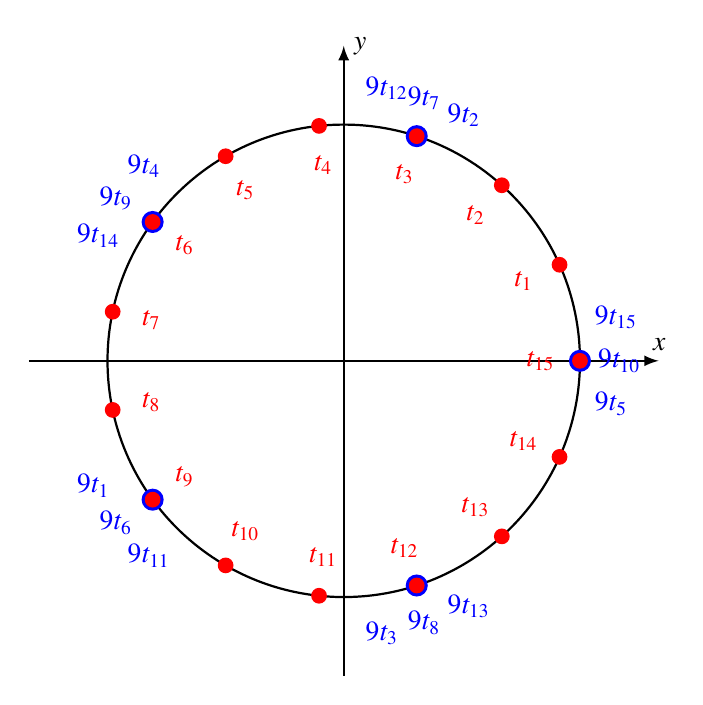
\begin{tikzpicture}[>=latex,thick]
\draw (0,0) circle[radius=3cm];
\draw[->] (-4,0)--(4,0) coordinate[label={$x$}];
\draw[->] (0,-4)--(0,4) coordinate[label={right:$y$}];
\foreach \j in {1,...,5}{
	\fill[color=blue] ({3 * cos(360 * \j/5)},{3 * sin(360 * \j/5)})
		circle[radius=0.14];
}
\def\N{15}
\foreach \j in {1,...,\N}{
	\fill[color=red] ({3 * cos(360 * \j/\N)},{3 * sin(360 * \j/\N})
		circle[radius=0.1];
	\node[color=red] at ({2.5*cos(\j*(360/\N))},{2.5*sin(\j*(360/\N))})
		{$t_{\j}$};
}
\def\k{9}
\pgfmathparse{\k*360/\N}
\xdef\a{\pgfmathresult}
\def\j{1}
\def\r{0.5}
\pgfmathparse{\j*\a-9}\xdef\aa{\pgfmathresult}
\node[color=blue] at ({3*cos(\aa)},{3*sin(\aa)})
	[shift={({\r*cos(\aa)},{\r*sin(\aa)})}] {$9t_{1\phantom{0}}$};
\def\j{2}
\pgfmathparse{\j*\a-9}\xdef\aa{\pgfmathresult}
\node[color=blue] at ({3*cos(\aa)},{3*sin(\aa)})
	[shift={({\r*cos(\aa)},{\r*sin(\aa)})}] {$9t_{2\phantom{0}}$};
\def\j{3}
\pgfmathparse{\j*\a-9}\xdef\aa{\pgfmathresult}
\node[color=blue] at ({3*cos(\aa)},{3*sin(\aa)})
	[shift={({\r*cos(\aa)},{\r*sin(\aa)})}] {$9t_{3\phantom{0}}$};
\def\j{4}
\pgfmathparse{\j*\a-9}\xdef\aa{\pgfmathresult}
\node[color=blue] at ({3*cos(\aa)},{3*sin(\aa)})
	[shift={({\r*cos(\aa)},{\r*sin(\aa)})}] {$9t_{4\phantom{0}}$};
\def\j{5}
\pgfmathparse{\j*\a-9}\xdef\aa{\pgfmathresult}
\node[color=blue] at ({3*cos(\aa)},{3*sin(\aa)})
	[shift={({\r*cos(\aa)},{\r*sin(\aa)})}] {$9t_{5\phantom{0}}$};
\def\j{6}
\pgfmathparse{\j*\a}\xdef\aa{\pgfmathresult}
\node[color=blue] at ({3*cos(\aa)},{3*sin(\aa)})
	[shift={({\r*cos(\aa)},{\r*sin(\aa)})}] {$9t_{6\phantom{0}}$};
\def\j{7}
\pgfmathparse{\j*\a}\xdef\aa{\pgfmathresult}
\node[color=blue] at ({3*cos(\aa)},{3*sin(\aa)})
	[shift={({\r*cos(\aa)},{\r*sin(\aa)})}] {$9t_{7\phantom{0}}$};
\def\j{8}
\pgfmathparse{\j*\a}\xdef\aa{\pgfmathresult}
\node[color=blue] at ({3*cos(\aa)},{3*sin(\aa)})
	[shift={({\r*cos(\aa)},{\r*sin(\aa)})}] {$9t_{8\phantom{0}}$};
\def\j{9}
\pgfmathparse{\j*\a}\xdef\aa{\pgfmathresult}
\node[color=blue] at ({3*cos(\aa)},{3*sin(\aa)})
	[shift={({\r*cos(\aa)},{\r*sin(\aa)})}] {$9t_{9\phantom{0}}$};
\def\j{10}
\pgfmathparse{\j*\a}\xdef\aa{\pgfmathresult}
\node[color=blue] at ({3*cos(\aa)},{3*sin(\aa)})
	[shift={({\r*cos(\aa)},{\r*sin(\aa)})}] {$9t_{10}$};
\def\j{11}
\pgfmathparse{\j*\a+9}\xdef\aa{\pgfmathresult}
\node[color=blue] at ({3*cos(\aa)},{3*sin(\aa)})
	[shift={({\r*cos(\aa)},{\r*sin(\aa)})}] {$9t_{11}$};
\def\j{12}
\pgfmathparse{\j*\a+9}\xdef\aa{\pgfmathresult}
\node[color=blue] at ({3*cos(\aa)},{3*sin(\aa)})
	[shift={({\r*cos(\aa)},{\r*sin(\aa)})}] {$9t_{12}$};
\def\j{13}
\pgfmathparse{\j*\a+9}\xdef\aa{\pgfmathresult}
\node[color=blue] at ({3*cos(\aa)},{3*sin(\aa)})
	[shift={({\r*cos(\aa)},{\r*sin(\aa)})}] {$9t_{13}$};
\def\j{14}
\pgfmathparse{\j*\a+9}\xdef\aa{\pgfmathresult}
\node[color=blue] at ({3*cos(\aa)},{3*sin(\aa)})
	[shift={({\r*cos(\aa)},{\r*sin(\aa)})}] {$9t_{14}$};
\def\j{15}
\pgfmathparse{\j*\a+9}\xdef\aa{\pgfmathresult}
\node[color=blue] at ({3*cos(\aa)},{3*sin(\aa)})
	[shift={({\r*cos(\aa)},{\r*sin(\aa)})}] {$9t_{15}$};

\end{tikzpicture}

\end{document}
